\appendix
\section*{Appendix}

\noindent There are three kinds of data used to generate this \textbf{\textcolor{coBalt}{Comprehensive Development Plan}}: community engagement data, socioeconomic data, and map and geospatial data. This appendix documents how these data were acquired, processed, and presented. Finally, it also summarizes the technical procedures used to generate the tangible document of the plan.

\section{Community Engagment Process}

\noindent Community and resident engagement is crucial to the Plan for several reasons:
\begin{enumerate}
    \item [(1)] \textbf{Inclusivity and Representation}: The Plan intends to address the needs and aspirations of the entire community. Including as many residents as possible ensures that a diverse range of voices and perspectives are heard and considered. This helps with efforts to reflect the values, priorities, and aspirations of the whole community.
    \item [(2)] \textbf{Local Knowledge and Expertise}: Local knowledge and input help to ground the Plan in the realities of the area. Residents have firsthand knowledge about their neighborhood and its unique characteristics. Their insights are invaluable to identifying specific needs and opportunities that would only be known by those who experience Bloomfield daily.
    \item [(3)] \textbf{Trust and Transparency}: Engaging residents in the planning process builds trust between the community and the municipal government. Transparent and inclusive decision-making processes foster greater confidence that the plan is responsive to community needs. This trust will build partnerships between residents, local government, and other stakeholders necessary to implement the Plan.
\end{enumerate}

\subsection{Bloomfield Community Engagement Process}
\noindent Residents, stakeholders, and advocates were engaged on \hl{N} separate occasions throughout the entire planning process.
\begin{enumerate}
    \item [(1)] \hl{[list of engagements]}
\end{enumerate}

\subsection{Community Engagement Kickoff}

\noindent The community engagement process began with identifying and inviting local stakeholders and advocates to assist with identifying priorities early in the process. A \textbf{\textcolor{coBalt}{stakeholder}} is any resident that has a vested interest in seeing Bloomfield grow as a community. An \textbf{\textcolor{coBalt}{advocate}} is any individual involved with the community that can speak up for stakeholders who are unable to participate in the community engagement process.\\

\noindent The consultant team hosted the kickoff on \hl{[date]} to provide an overview of the planning process and invite attendants to participate in a model building and consensus workshop scheduled in November 2023.

\subsection{Model Building and Consensus Workshop}

\noindent On November 7, 2023, Bloomfield residents, stakeholders, and advocates attended a community consensus workshop facilitated by community and economic development consultants with FIVE RULE Rural Planning of Kearney, NE. Lowell Schroeder and Bobbi Pettit facilitated a conversation among roughly 50 members of the Bloomfield Community.

\subsubsection*{Model Building Introductions}
\noindent Attendees introduced themselves through an inclusive participatory process that asked each participant to remember a time when he or she felt very happy, safe, and proud to be a member of the Bloomfield Community. They were then asked to select a random found object and use that object to describe the memory. Each participant introduced themselves, described their relationship to the Bloomfield Community, and described their object and memory. Every attendee shared a positive memory.\\

\noindent The ToP Consensus Workshop Method was utilized to assist attendees with identifying themes and creating a shared vision for the next decade in Bloomfield. The group was asked \textit{“What is needed now to make Bloomfield Better?"}\\

\noindent Each participant brainstormed immediate ideas (3 to 5 words) that came to mind when asked this question and then worked together with their tablemates to sort and organize the ideas. Ideas were then combined and sorted on a shared wall. This exercise ultimately led to the themes addressed in the eventual community survey.\\

\subsection*{Workshop themes}

\noindent \hl{[insert image of workshop themes HERE]}

\subsection{Communitywide Survey}

\noindent The themes that rose to the surface because of the workshop were utilized to create a survey made available to the entire Bloomfield community \hl{[in Spring 2024]}. Survey responses are reported throughout the plan where appropriate.\\

\noindent The survey was made available in both online and paper copy formats. 162 respondents participated in the survey.

\begin{figure}[ht!]
\centering
\begin{framed}
    \caption{Community Survey Neighborhoods}
    \label{fig:neighborhoods}

     \begin{subfigure}{0.49\textwidth}
        \centering
        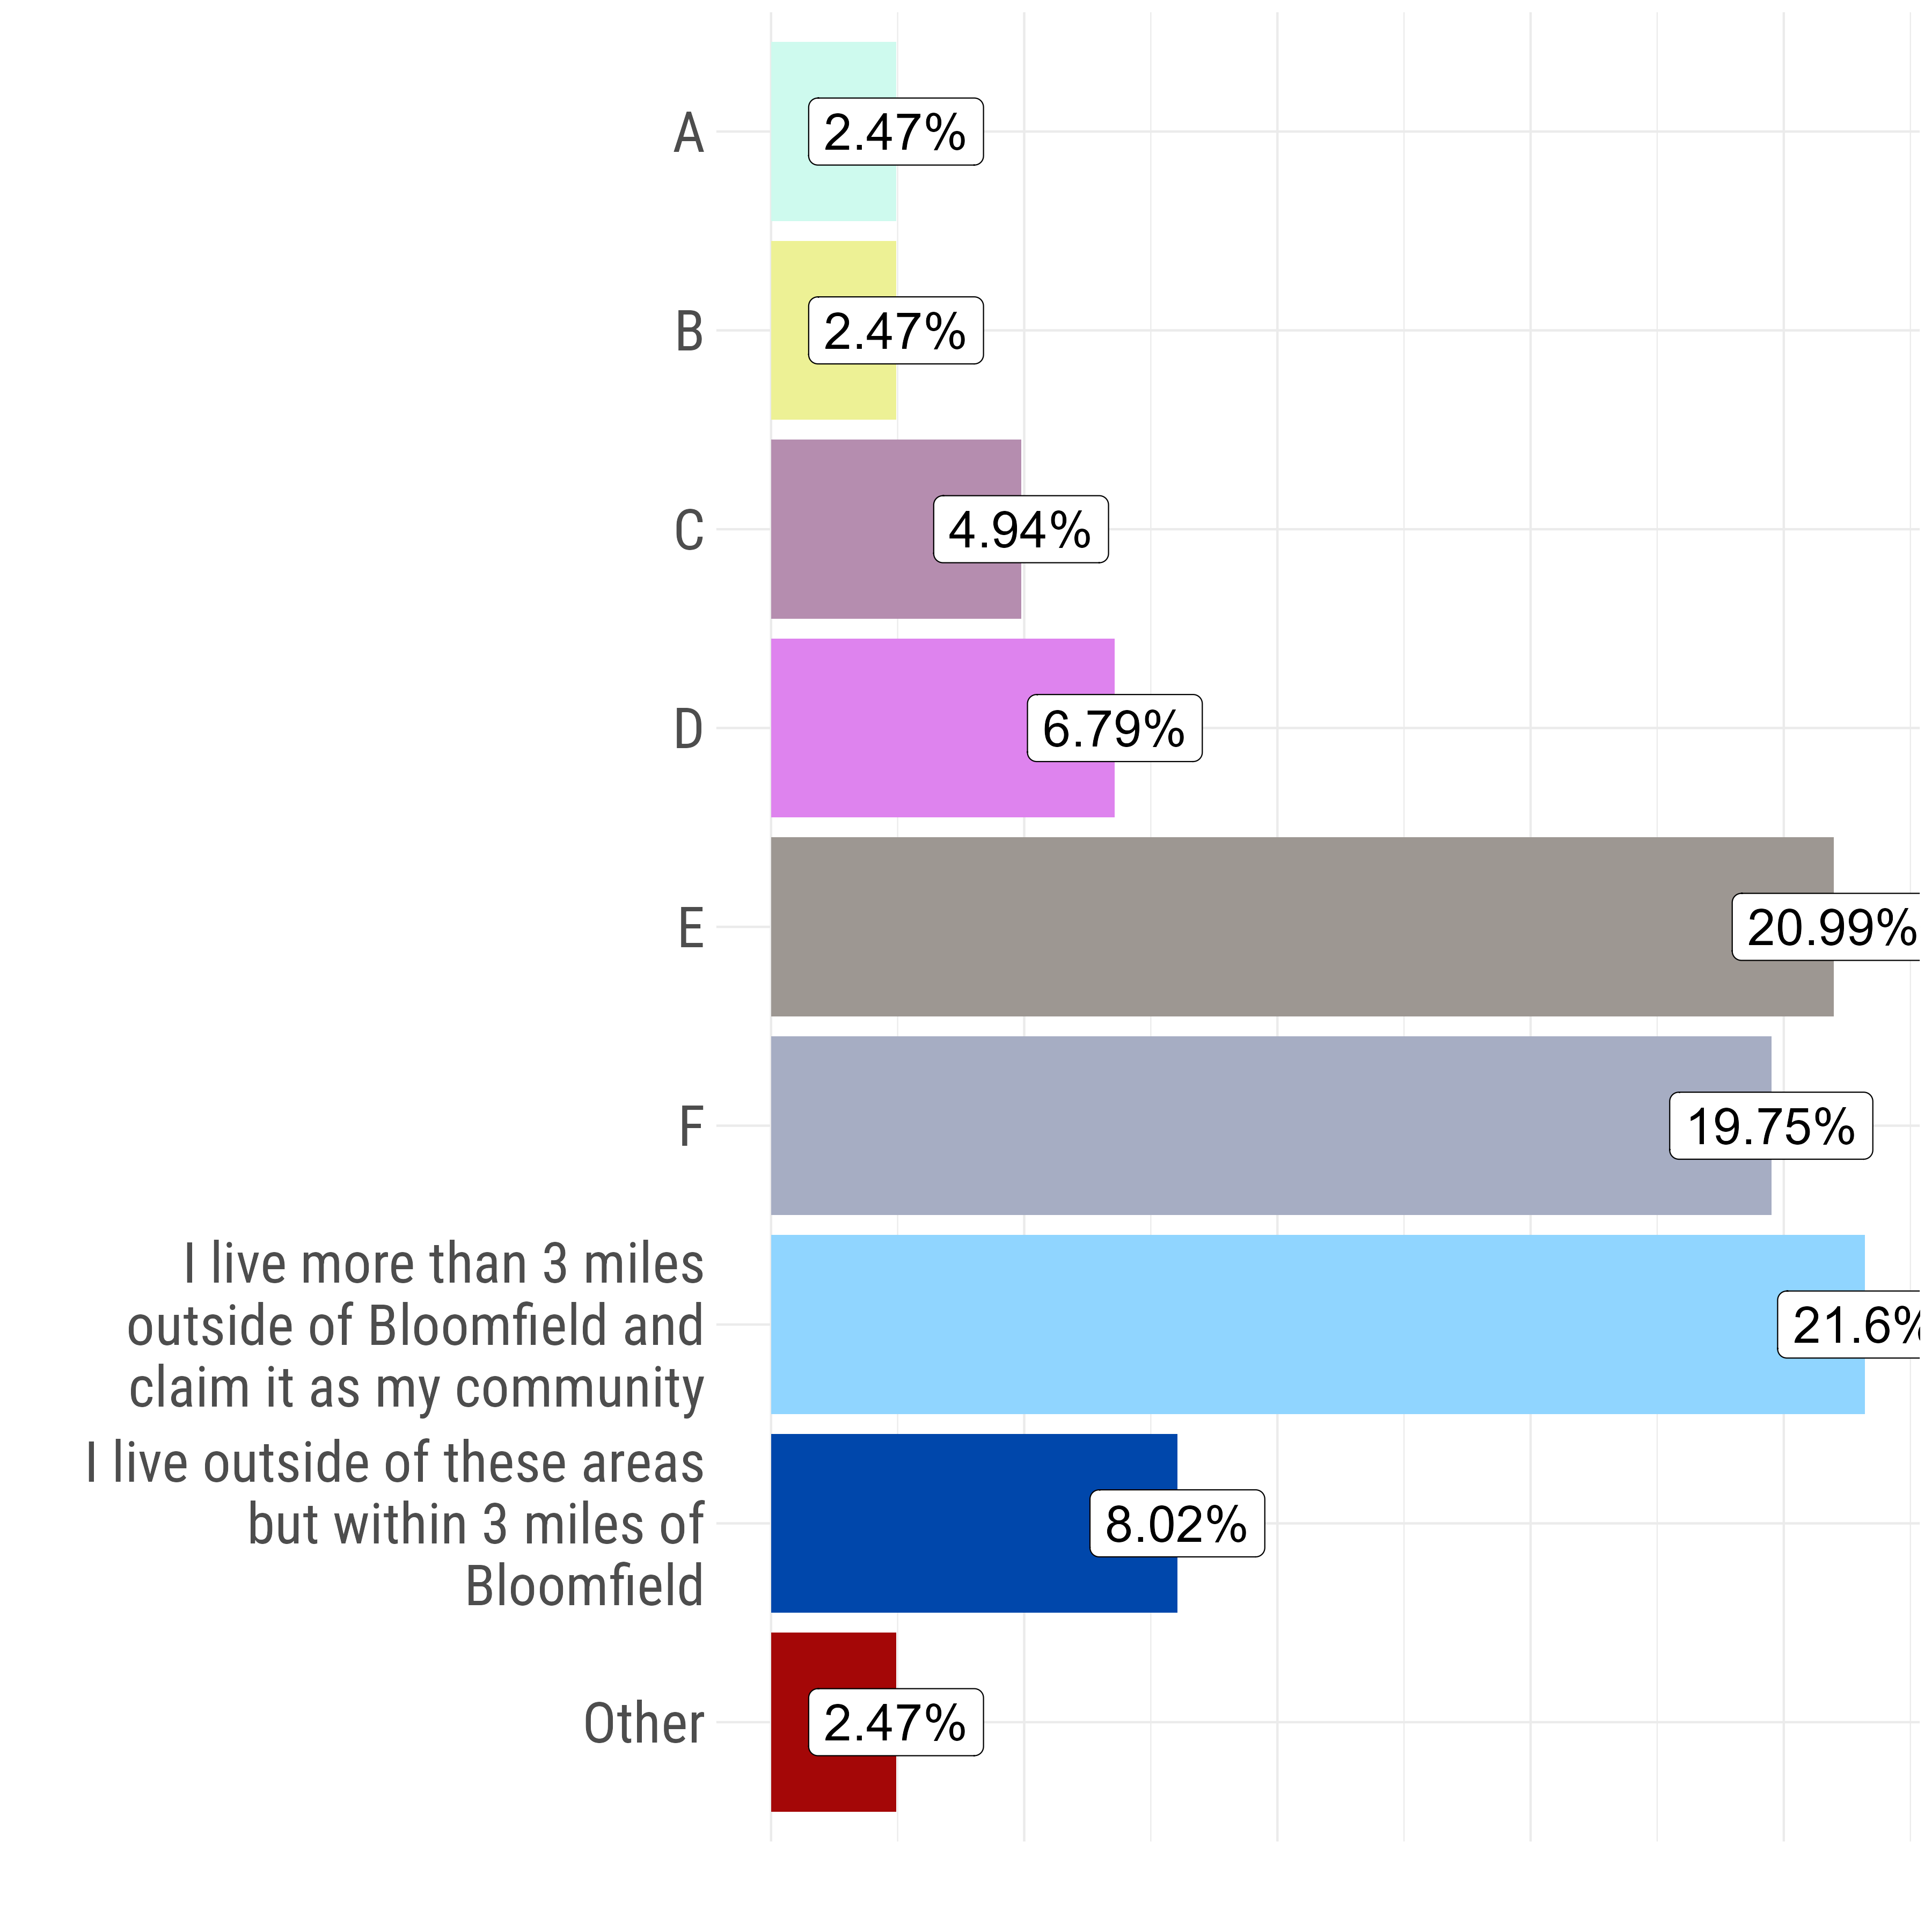
\includegraphics[width=\linewidth]{figures/survey_respondent_neighborhoods.png}
     \end{subfigure}
     \begin{subfigure}{0.49\textwidth}
        \centering
        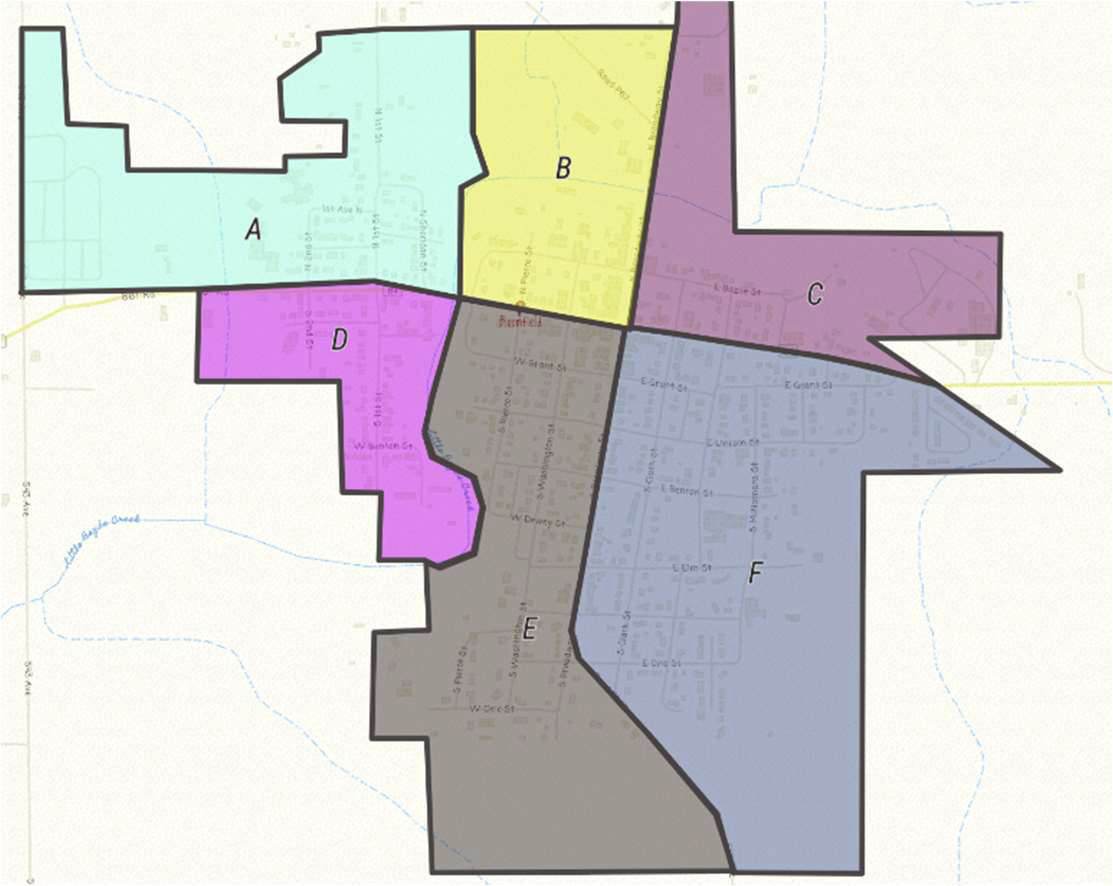
\includegraphics[width=\linewidth]{figures/community_survey_neighborhoods.png}
     \end{subfigure}
\end{framed}
\end{figure}

\noindent \hl{[survey summary toplines HERE]}

\pagebreak
\subsection{Future Land Use Map Workshop}

\noindent \hl{[is the online discussion on September 8 2025 the only one?]}

\section{Socioeconomic Data Curation}

\section{Map Development}

\section{Document Generation}

